\documentclass[1p]{elsarticle_modified}
%\bibliographystyle{elsarticle-num}

%\usepackage[colorlinks]{hyperref}
%\usepackage{abbrmath_seonhwa} %\Abb, \Ascr, \Acal ,\Abf, \Afrak
\usepackage{amsfonts}
\usepackage{amssymb}
\usepackage{amsmath}
\usepackage{amsthm}
\usepackage{scalefnt}
\usepackage{amsbsy}
\usepackage{kotex}
\usepackage{caption}
\usepackage{subfig}
\usepackage{color}
\usepackage{graphicx}
\usepackage{xcolor} %% white, black, red, green, blue, cyan, magenta, yellow
\usepackage{float}
\usepackage{setspace}
\usepackage{hyperref}

\usepackage{tikz}
\usetikzlibrary{arrows}

\usepackage{multirow}
\usepackage{array} % fixed length table
\usepackage{hhline}

%%%%%%%%%%%%%%%%%%%%%
\makeatletter
\renewcommand*\env@matrix[1][\arraystretch]{%
	\edef\arraystretch{#1}%
	\hskip -\arraycolsep
	\let\@ifnextchar\new@ifnextchar
	\array{*\c@MaxMatrixCols c}}
\makeatother %https://tex.stackexchange.com/questions/14071/how-can-i-increase-the-line-spacing-in-a-matrix
%%%%%%%%%%%%%%%

\usepackage[normalem]{ulem}

\newcommand{\msout}[1]{\ifmmode\text{\sout{\ensuremath{#1}}}\else\sout{#1}\fi}
%SOURCE: \msout is \stkout macro in https://tex.stackexchange.com/questions/20609/strikeout-in-math-mode

\newcommand{\cancel}[1]{
	\ifmmode
	{\color{red}\msout{#1}}
	\else
	{\color{red}\sout{#1}}
	\fi
}

\newcommand{\add}[1]{
	{\color{blue}\uwave{#1}}
}

\newcommand{\replace}[2]{
	\ifmmode
	{\color{red}\msout{#1}}{\color{blue}\uwave{#2}}
	\else
	{\color{red}\sout{#1}}{\color{blue}\uwave{#2}}
	\fi
}

\newcommand{\Sol}{\mathcal{S}} %segment
\newcommand{\D}{D} %diagram
\newcommand{\A}{\mathcal{A}} %arc


%%%%%%%%%%%%%%%%%%%%%%%%%%%%%5 test

\def\sl{\operatorname{\textup{SL}}(2,\Cbb)}
\def\psl{\operatorname{\textup{PSL}}(2,\Cbb)}
\def\quan{\mkern 1mu \triangleright \mkern 1mu}

\theoremstyle{definition}
\newtheorem{thm}{Theorem}[section]
\newtheorem{prop}[thm]{Proposition}
\newtheorem{lem}[thm]{Lemma}
\newtheorem{ques}[thm]{Question}
\newtheorem{cor}[thm]{Corollary}
\newtheorem{defn}[thm]{Definition}
\newtheorem{exam}[thm]{Example}
\newtheorem{rmk}[thm]{Remark}
\newtheorem{alg}[thm]{Algorithm}

\newcommand{\I}{\sqrt{-1}}
\begin{document}

%\begin{frontmatter}
%
%\title{Boundary parabolic representations of knots up to 8 crossings}
%
%%% Group authors per affiliation:
%\author{Yunhi Cho} 
%\address{Department of Mathematics, University of Seoul, Seoul, Korea}
%\ead{yhcho@uos.ac.kr}
%
%
%\author{Seonhwa Kim} %\fnref{s_kim}}
%\address{Center for Geometry and Physics, Institute for Basic Science, Pohang, 37673, Korea}
%\ead{ryeona17@ibs.re.kr}
%
%\author{Hyuk Kim}
%\address{Department of Mathematical Sciences, Seoul National University, Seoul 08826, Korea}
%\ead{hyukkim@snu.ac.kr}
%
%\author{Seokbeom Yoon}
%\address{Department of Mathematical Sciences, Seoul National University, Seoul, 08826,  Korea}
%\ead{sbyoon15@snu.ac.kr}
%
%\begin{abstract}
%We find all boundary parabolic representation of knots up to 8 crossings.
%
%\end{abstract}
%\begin{keyword}
%    \MSC[2010] 57M25 
%\end{keyword}
%
%\end{frontmatter}

%\linenumbers
%\tableofcontents
%
\newcommand\colored[1]{\textcolor{white}{\rule[-0.35ex]{0.8em}{1.4ex}}\kern-0.8em\color{red} #1}%
%\newcommand\colored[1]{\textcolor{white}{ #1}\kern-2.17ex	\textcolor{white}{ #1}\kern-1.81ex	\textcolor{white}{ #1}\kern-2.15ex\color{red}#1	}

{\Large $\underline{12n_{0180}~(K12n_{0180})}$}

\setlength{\tabcolsep}{10pt}
\renewcommand{\arraystretch}{1.6}
\vspace{1cm}\begin{tabular}{m{100pt}>{\centering\arraybackslash}m{274pt}}
\multirow{5}{120pt}{
	\centering
	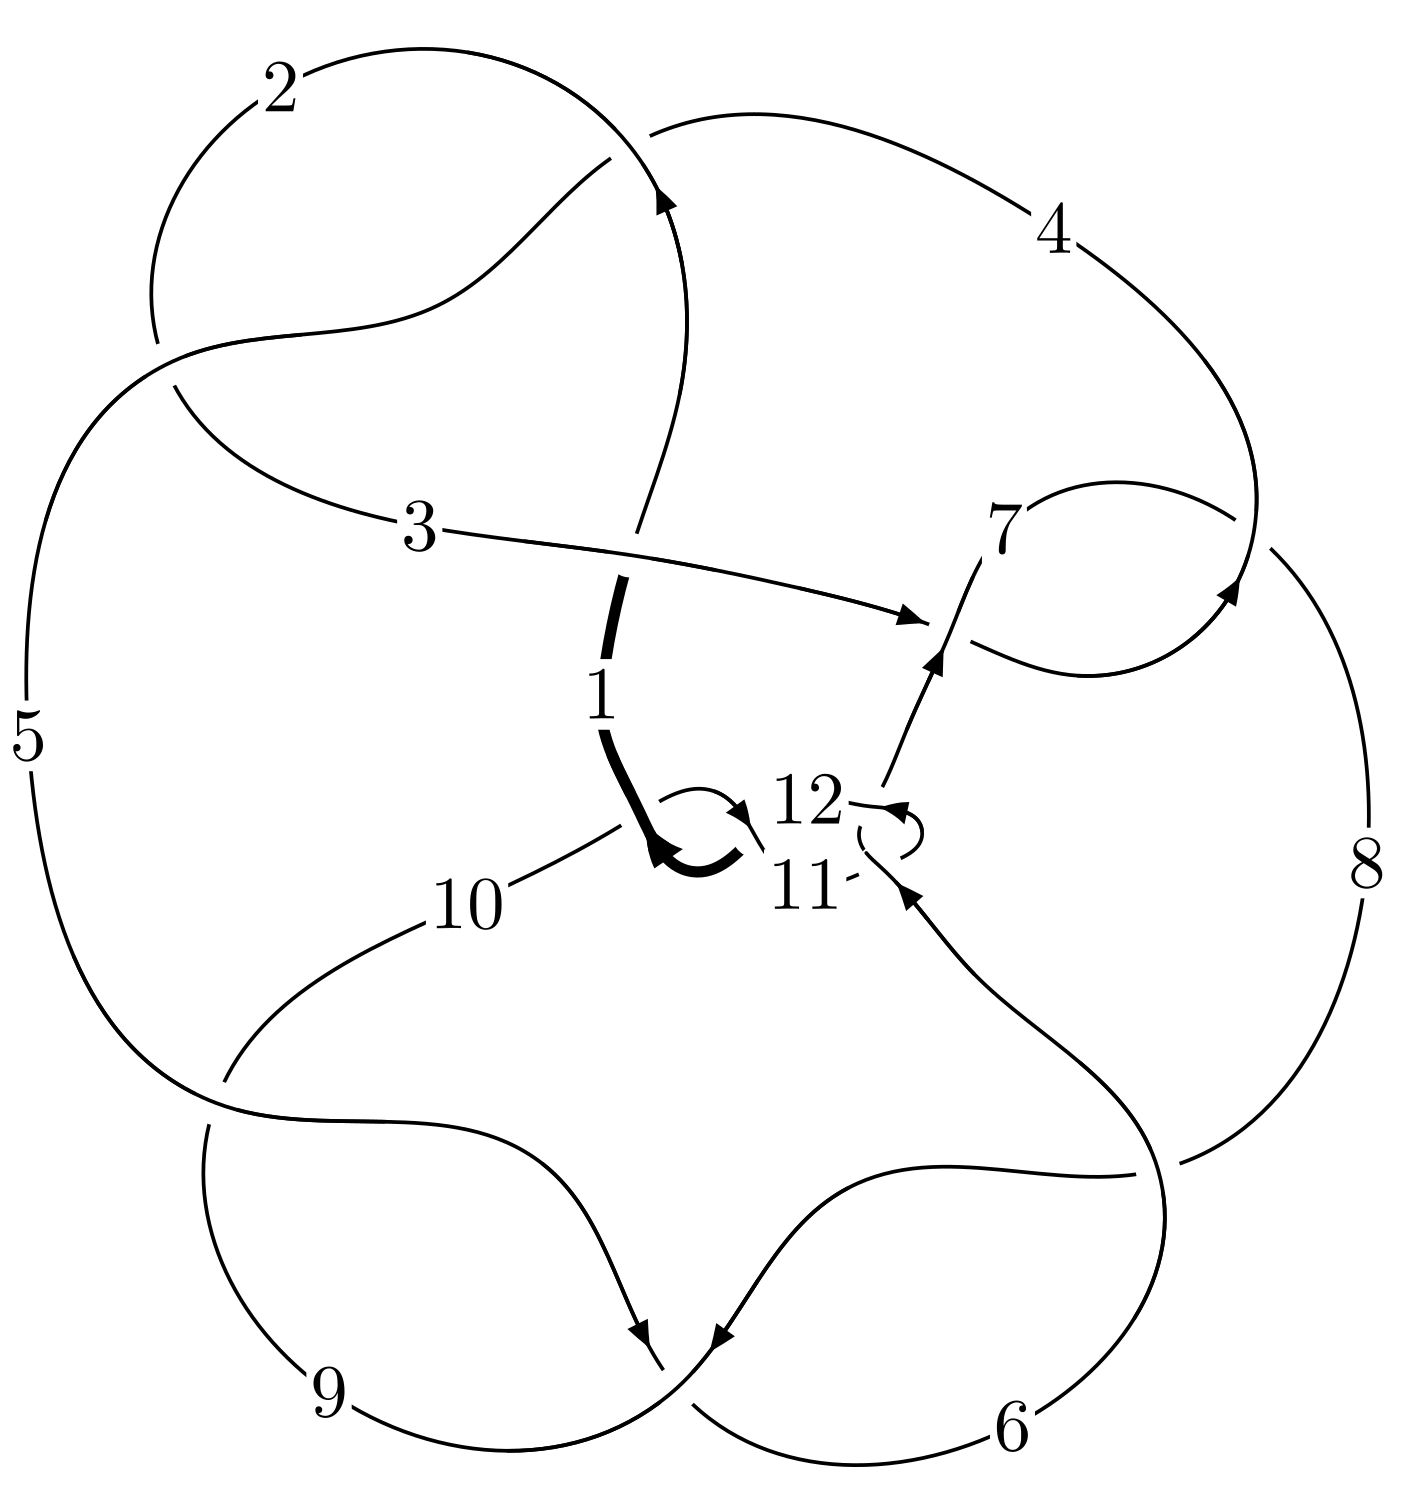
\includegraphics[width=112pt]{../../../GIT/diagram.site/Diagrams/png/2269_12n_0180.png}\\
\ \ \ A knot diagram\footnotemark}&
\allowdisplaybreaks
\textbf{Linearized knot diagam} \\
\cline{2-2}
 &
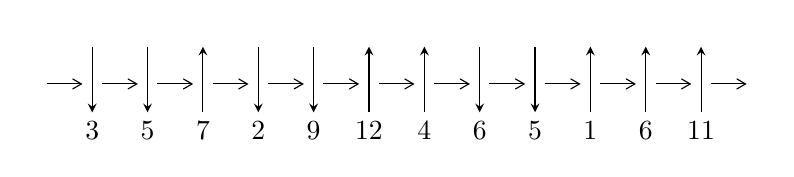
\begin{tikzpicture}[x=20pt, y=17pt]
	% nodes
	\node (C0) at (0, 0) {};
	\node (C1) at (1, 0) {};
	\node (C1U) at (1, +1) {};
	\node (C1D) at (1, -1) {3};

	\node (C2) at (2, 0) {};
	\node (C2U) at (2, +1) {};
	\node (C2D) at (2, -1) {5};

	\node (C3) at (3, 0) {};
	\node (C3U) at (3, +1) {};
	\node (C3D) at (3, -1) {7};

	\node (C4) at (4, 0) {};
	\node (C4U) at (4, +1) {};
	\node (C4D) at (4, -1) {2};

	\node (C5) at (5, 0) {};
	\node (C5U) at (5, +1) {};
	\node (C5D) at (5, -1) {9};

	\node (C6) at (6, 0) {};
	\node (C6U) at (6, +1) {};
	\node (C6D) at (6, -1) {12};

	\node (C7) at (7, 0) {};
	\node (C7U) at (7, +1) {};
	\node (C7D) at (7, -1) {4};

	\node (C8) at (8, 0) {};
	\node (C8U) at (8, +1) {};
	\node (C8D) at (8, -1) {6};

	\node (C9) at (9, 0) {};
	\node (C9U) at (9, +1) {};
	\node (C9D) at (9, -1) {5};

	\node (C10) at (10, 0) {};
	\node (C10U) at (10, +1) {};
	\node (C10D) at (10, -1) {1};

	\node (C11) at (11, 0) {};
	\node (C11U) at (11, +1) {};
	\node (C11D) at (11, -1) {6};

	\node (C12) at (12, 0) {};
	\node (C12U) at (12, +1) {};
	\node (C12D) at (12, -1) {11};
	\node (C13) at (13, 0) {};

	% arrows
	\draw[->,>={angle 60}]
	(C0) edge (C1) (C1) edge (C2) (C2) edge (C3) (C3) edge (C4) (C4) edge (C5) (C5) edge (C6) (C6) edge (C7) (C7) edge (C8) (C8) edge (C9) (C9) edge (C10) (C10) edge (C11) (C11) edge (C12) (C12) edge (C13) ;	\draw[->,>=stealth]
	(C1U) edge (C1D) (C2U) edge (C2D) (C3D) edge (C3U) (C4U) edge (C4D) (C5U) edge (C5D) (C6D) edge (C6U) (C7D) edge (C7U) (C8U) edge (C8D) (C9U) edge (C9D) (C10D) edge (C10U) (C11D) edge (C11U) (C12D) edge (C12U) ;
	\end{tikzpicture} \\
\hhline{~~} \\& 
\textbf{Solving Sequence} \\ \cline{2-2} 
 &
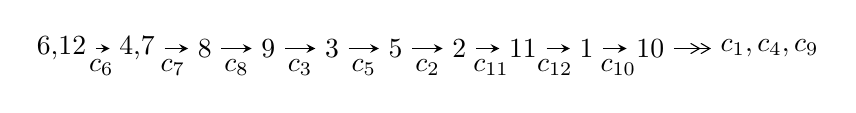
\begin{tikzpicture}[x=23pt, y=7pt]
	% node
	\node (A0) at (-1/8, 0) {6,12};
	\node (A1) at (17/16, 0) {4,7};
	\node (A2) at (17/8, 0) {8};
	\node (A3) at (25/8, 0) {9};
	\node (A4) at (33/8, 0) {3};
	\node (A5) at (41/8, 0) {5};
	\node (A6) at (49/8, 0) {2};
	\node (A7) at (57/8, 0) {11};
	\node (A8) at (65/8, 0) {1};
	\node (A9) at (73/8, 0) {10};
	\node (C1) at (1/2, -1) {$c_{6}$};
	\node (C2) at (13/8, -1) {$c_{7}$};
	\node (C3) at (21/8, -1) {$c_{8}$};
	\node (C4) at (29/8, -1) {$c_{3}$};
	\node (C5) at (37/8, -1) {$c_{5}$};
	\node (C6) at (45/8, -1) {$c_{2}$};
	\node (C7) at (53/8, -1) {$c_{11}$};
	\node (C8) at (61/8, -1) {$c_{12}$};
	\node (C9) at (69/8, -1) {$c_{10}$};
	\node (A10) at (11, 0) {$c_{1},c_{4},c_{9}$};

	% edge
	\draw[->,>=stealth]	
	(A0) edge (A1) (A1) edge (A2) (A2) edge (A3) (A3) edge (A4) (A4) edge (A5) (A5) edge (A6) (A6) edge (A7) (A7) edge (A8) (A8) edge (A9) ;
	\draw[->>,>={angle 60}]	
	(A9) edge (A10);
\end{tikzpicture} \\ 

\end{tabular} \\

\footnotetext{
The image of knot diagram is generated by the software ``\textbf{Draw programme}" developed by Andrew Bartholomew(\url{http://www.layer8.co.uk/maths/draw/index.htm\#Running-draw}), where we modified some parts for our purpose(\url{https://github.com/CATsTAILs/LinksPainter}).
}\phantom \\ \newline 
\centering \textbf{Ideals for irreducible components\footnotemark of $X_{\text{par}}$} 
 
\begin{align*}
I^u_{1}&=\langle 
8.59216\times10^{59} u^{59}+7.11341\times10^{60} u^{58}+\cdots+2.71076\times10^{61} b+6.33557\times10^{61},\\
\phantom{I^u_{1}}&\phantom{= \langle  }-2.02586\times10^{62} u^{59}-3.30298\times10^{62} u^{58}+\cdots+4.60829\times10^{62} a-1.81464\times10^{63},\\
\phantom{I^u_{1}}&\phantom{= \langle  }u^{60}+3 u^{59}+\cdots+12 u+17\rangle \\
I^u_{2}&=\langle 
-51 u^3 a^2+106 u^3 a+\cdots-80 a-21,\\
\phantom{I^u_{2}}&\phantom{= \langle  }-2 u^3 a^2-2 a^2 u^2+u^3 a+a^3+a^2 u+2 u^2 a+6 u^3+2 a^2-3 a u+9 u^2-2 a+2 u-2,\;u^4- u^2+1\rangle \\
\\
\end{align*}
\raggedright * 2 irreducible components of $\dim_{\mathbb{C}}=0$, with total 72 representations.\\
\footnotetext{All coefficients of polynomials are rational numbers. But the coefficients are sometimes approximated in decimal forms when there is not enough margin.}
\newpage
\renewcommand{\arraystretch}{1}
\centering \section*{I. $I^u_{1}= \langle 8.59\times10^{59} u^{59}+7.11\times10^{60} u^{58}+\cdots+2.71\times10^{61} b+6.34\times10^{61},\;-2.03\times10^{62} u^{59}-3.30\times10^{62} u^{58}+\cdots+4.61\times10^{62} a-1.81\times10^{63},\;u^{60}+3 u^{59}+\cdots+12 u+17 \rangle$}
\flushleft \textbf{(i) Arc colorings}\\
\begin{tabular}{m{7pt} m{180pt} m{7pt} m{180pt} }
\flushright $a_{6}=$&$\begin{pmatrix}1\\0\end{pmatrix}$ \\
\flushright $a_{12}=$&$\begin{pmatrix}0\\u\end{pmatrix}$ \\
\flushright $a_{4}=$&$\begin{pmatrix}0.439611 u^{59}+0.716748 u^{58}+\cdots-0.813297 u+3.93778\\-0.0316965 u^{59}-0.262414 u^{58}+\cdots+4.37519 u-2.33720\end{pmatrix}$ \\
\flushright $a_{7}=$&$\begin{pmatrix}1\\- u^2\end{pmatrix}$ \\
\flushright $a_{8}=$&$\begin{pmatrix}0.0820681 u^{59}+0.302588 u^{58}+\cdots-10.8701 u-5.50752\\-0.0713087 u^{59}-0.287800 u^{58}+\cdots+3.92724 u+1.83826\end{pmatrix}$ \\
\flushright $a_{9}=$&$\begin{pmatrix}0.153377 u^{59}+0.590388 u^{58}+\cdots-14.7973 u-7.34578\\-0.0713087 u^{59}-0.287800 u^{58}+\cdots+3.92724 u+1.83826\end{pmatrix}$ \\
\flushright $a_{3}=$&$\begin{pmatrix}0.106413 u^{59}+0.119118 u^{58}+\cdots-4.94013 u-3.96049\\0.0147849 u^{59}+0.000149588 u^{58}+\cdots+3.53440 u+4.49621\end{pmatrix}$ \\
\flushright $a_{5}=$&$\begin{pmatrix}-0.313827 u^{59}-0.803067 u^{58}+\cdots+2.00850 u-0.850375\\-0.0119731 u^{59}-0.0516958 u^{58}+\cdots+2.55197 u+2.41305\end{pmatrix}$ \\
\flushright $a_{2}=$&$\begin{pmatrix}0.111888 u^{59}+0.442512 u^{58}+\cdots-5.49722 u-3.98640\\0.0511739 u^{59}+0.197997 u^{58}+\cdots-3.04177 u+1.75645\end{pmatrix}$ \\
\flushright $a_{11}=$&$\begin{pmatrix}- u\\u\end{pmatrix}$ \\
\flushright $a_{1}=$&$\begin{pmatrix}u^3\\- u^3+u\end{pmatrix}$ \\
\flushright $a_{10}=$&$\begin{pmatrix}- u^5- u\\u^5- u^3+u\end{pmatrix}$\\&\end{tabular}
\flushleft \textbf{(ii) Obstruction class $= -1$}\\~\\
\flushleft \textbf{(iii) Cusp Shapes $= 0.359408 u^{59}+0.109275 u^{58}+\cdots+23.9102 u+7.48289$}\\~\\
\newpage\renewcommand{\arraystretch}{1}
\flushleft \textbf{(iv) u-Polynomials at the component}\newline \\
\begin{tabular}{m{50pt}|m{274pt}}
Crossings & \hspace{64pt}u-Polynomials at each crossing \\
\hline $$\begin{aligned}c_{1}\end{aligned}$$&$\begin{aligned}
&u^{60}+35 u^{59}+\cdots+64 u+1
\end{aligned}$\\
\hline $$\begin{aligned}c_{2},c_{4}\end{aligned}$$&$\begin{aligned}
&u^{60}-5 u^{59}+\cdots-16 u+1
\end{aligned}$\\
\hline $$\begin{aligned}c_{3},c_{7}\end{aligned}$$&$\begin{aligned}
&u^{60}- u^{59}+\cdots-4 u+1
\end{aligned}$\\
\hline $$\begin{aligned}c_{5},c_{8},c_{9}\end{aligned}$$&$\begin{aligned}
&u^{60}-3 u^{59}+\cdots-154 u+49
\end{aligned}$\\
\hline $$\begin{aligned}c_{6},c_{11}\end{aligned}$$&$\begin{aligned}
&u^{60}-3 u^{59}+\cdots-12 u+17
\end{aligned}$\\
\hline $$\begin{aligned}c_{10},c_{12}\end{aligned}$$&$\begin{aligned}
&u^{60}-17 u^{59}+\cdots-2558 u+289
\end{aligned}$\\
\hline
\end{tabular}\\~\\
\newpage\renewcommand{\arraystretch}{1}
\flushleft \textbf{(v) Riley Polynomials at the component}\newline \\
\begin{tabular}{m{50pt}|m{274pt}}
Crossings & \hspace{64pt}Riley Polynomials at each crossing \\
\hline $$\begin{aligned}c_{1}\end{aligned}$$&$\begin{aligned}
&y^{60}-15 y^{59}+\cdots+2064 y+1
\end{aligned}$\\
\hline $$\begin{aligned}c_{2},c_{4}\end{aligned}$$&$\begin{aligned}
&y^{60}-35 y^{59}+\cdots-64 y+1
\end{aligned}$\\
\hline $$\begin{aligned}c_{3},c_{7}\end{aligned}$$&$\begin{aligned}
&y^{60}-15 y^{59}+\cdots-40 y+1
\end{aligned}$\\
\hline $$\begin{aligned}c_{5},c_{8},c_{9}\end{aligned}$$&$\begin{aligned}
&y^{60}+21 y^{59}+\cdots+34104 y+2401
\end{aligned}$\\
\hline $$\begin{aligned}c_{6},c_{11}\end{aligned}$$&$\begin{aligned}
&y^{60}-17 y^{59}+\cdots-2558 y+289
\end{aligned}$\\
\hline $$\begin{aligned}c_{10},c_{12}\end{aligned}$$&$\begin{aligned}
&y^{60}+59 y^{59}+\cdots-725794 y+83521
\end{aligned}$\\
\hline
\end{tabular}\\~\\
\newpage\flushleft \textbf{(vi) Complex Volumes and Cusp Shapes}
$$\begin{array}{c|c|c}  
\text{Solutions to }I^u_{1}& \I (\text{vol} + \sqrt{-1}CS) & \text{Cusp shape}\\
 \hline 
\begin{aligned}
u &= \phantom{-}0.929012 + 0.409111 I \\
a &= -3.04269 + 1.15379 I \\
b &= \phantom{-}2.59631 + 1.09970 I\end{aligned}
 & -0.23119 + 1.94297 I & -2.05685 - 11.08290 I \\ \hline\begin{aligned}
u &= \phantom{-}0.929012 - 0.409111 I \\
a &= -3.04269 - 1.15379 I \\
b &= \phantom{-}2.59631 - 1.09970 I\end{aligned}
 & -0.23119 - 1.94297 I & -2.05685 + 11.08290 I \\ \hline\begin{aligned}
u &= -0.832822 + 0.587944 I \\
a &= -1.21567 - 1.08428 I \\
b &= \phantom{-}0.069828 - 1.012120 I\end{aligned}
 & \phantom{-}3.25865 + 0.70404 I & -1.90677 + 0.77167 I \\ \hline\begin{aligned}
u &= -0.832822 - 0.587944 I \\
a &= -1.21567 + 1.08428 I \\
b &= \phantom{-}0.069828 + 1.012120 I\end{aligned}
 & \phantom{-}3.25865 - 0.70404 I & -1.90677 - 0.77167 I \\ \hline\begin{aligned}
u &= \phantom{-}0.004950 + 1.024030 I \\
a &= \phantom{-}0.183534 - 0.050087 I \\
b &= \phantom{-}0.740563 - 0.693298 I\end{aligned}
 & -3.25466 - 4.08265 I & -4.68553 + 7.94094 I \\ \hline\begin{aligned}
u &= \phantom{-}0.004950 - 1.024030 I \\
a &= \phantom{-}0.183534 + 0.050087 I \\
b &= \phantom{-}0.740563 + 0.693298 I\end{aligned}
 & -3.25466 + 4.08265 I & -4.68553 - 7.94094 I \\ \hline\begin{aligned}
u &= -0.822970 + 0.630204 I \\
a &= \phantom{-}1.54004 + 1.13008 I \\
b &= -0.133459 + 1.061150 I\end{aligned}
 & \phantom{-}3.19637 - 5.46860 I & -1.43660 + 7.42023 I \\ \hline\begin{aligned}
u &= -0.822970 - 0.630204 I \\
a &= \phantom{-}1.54004 - 1.13008 I \\
b &= -0.133459 - 1.061150 I\end{aligned}
 & \phantom{-}3.19637 + 5.46860 I & -1.43660 - 7.42023 I \\ \hline\begin{aligned}
u &= \phantom{-}0.809567 + 0.501021 I \\
a &= -5.62494 - 3.66221 I \\
b &= -0.98200 + 6.14395 I\end{aligned}
 & -0.08137 + 2.05589 I & \phantom{-}27.6617 + 22.2084 I \\ \hline\begin{aligned}
u &= \phantom{-}0.809567 - 0.501021 I \\
a &= -5.62494 + 3.66221 I \\
b &= -0.98200 - 6.14395 I\end{aligned}
 & -0.08137 - 2.05589 I & \phantom{-}27.6617 - 22.2084 I\\
 \hline 
 \end{array}$$\newpage$$\begin{array}{c|c|c}  
\text{Solutions to }I^u_{1}& \I (\text{vol} + \sqrt{-1}CS) & \text{Cusp shape}\\
 \hline 
\begin{aligned}
u &= -1.006930 + 0.332122 I \\
a &= -1.315940 - 0.433014 I \\
b &= \phantom{-}0.99469 - 1.18965 I\end{aligned}
 & \phantom{-}0.04819 - 3.77072 I & \phantom{-}0.50249 + 5.64131 I \\ \hline\begin{aligned}
u &= -1.006930 - 0.332122 I \\
a &= -1.315940 + 0.433014 I \\
b &= \phantom{-}0.99469 + 1.18965 I\end{aligned}
 & \phantom{-}0.04819 + 3.77072 I & \phantom{-}0.50249 - 5.64131 I \\ \hline\begin{aligned}
u &= -1.079450 + 0.120285 I \\
a &= -1.043550 - 0.134913 I \\
b &= \phantom{-}0.563555 - 0.123402 I\end{aligned}
 & \phantom{-}1.73585 - 0.04165 I & \phantom{-}7.02929 - 1.55117 I \\ \hline\begin{aligned}
u &= -1.079450 - 0.120285 I \\
a &= -1.043550 + 0.134913 I \\
b &= \phantom{-}0.563555 + 0.123402 I\end{aligned}
 & \phantom{-}1.73585 + 0.04165 I & \phantom{-}7.02929 + 1.55117 I \\ \hline\begin{aligned}
u &= -0.931671 + 0.569277 I \\
a &= \phantom{-}0.339977 + 1.097140 I \\
b &= -0.986373 - 0.325235 I\end{aligned}
 & \phantom{-}1.83197 - 2.08769 I & \phantom{-}7.31144 + 2.76134 I \\ \hline\begin{aligned}
u &= -0.931671 - 0.569277 I \\
a &= \phantom{-}0.339977 - 1.097140 I \\
b &= -0.986373 + 0.325235 I\end{aligned}
 & \phantom{-}1.83197 + 2.08769 I & \phantom{-}7.31144 - 2.76134 I \\ \hline\begin{aligned}
u &= \phantom{-}1.085650 + 0.220553 I \\
a &= \phantom{-}2.03983 + 0.42897 I \\
b &= -1.19988 - 0.96562 I\end{aligned}
 & \phantom{-}3.75827 + 4.28418 I & \phantom{-}7.39769 - 5.27258 I \\ \hline\begin{aligned}
u &= \phantom{-}1.085650 - 0.220553 I \\
a &= \phantom{-}2.03983 - 0.42897 I \\
b &= -1.19988 + 0.96562 I\end{aligned}
 & \phantom{-}3.75827 - 4.28418 I & \phantom{-}7.39769 + 5.27258 I \\ \hline\begin{aligned}
u &= -0.758636 + 0.887275 I \\
a &= -0.340815 - 0.278642 I \\
b &= -0.78502 - 1.49028 I\end{aligned}
 & -3.82130 + 3.76339 I & \phantom{-0.000000 } 0 \\ \hline\begin{aligned}
u &= -0.758636 - 0.887275 I \\
a &= -0.340815 + 0.278642 I \\
b &= -0.78502 + 1.49028 I\end{aligned}
 & -3.82130 - 3.76339 I & \phantom{-0.000000 } 0\\
 \hline 
 \end{array}$$\newpage$$\begin{array}{c|c|c}  
\text{Solutions to }I^u_{1}& \I (\text{vol} + \sqrt{-1}CS) & \text{Cusp shape}\\
 \hline 
\begin{aligned}
u &= \phantom{-}0.802241 + 0.075713 I \\
a &= \phantom{-}2.17404 - 1.63873 I \\
b &= -0.323287 + 0.783361 I\end{aligned}
 & \phantom{-}6.00487 - 2.27473 I & \phantom{-}9.19193 + 3.71392 I \\ \hline\begin{aligned}
u &= \phantom{-}0.802241 - 0.075713 I \\
a &= \phantom{-}2.17404 + 1.63873 I \\
b &= -0.323287 - 0.783361 I\end{aligned}
 & \phantom{-}6.00487 + 2.27473 I & \phantom{-}9.19193 - 3.71392 I \\ \hline\begin{aligned}
u &= \phantom{-}0.879342 + 0.837979 I \\
a &= -0.176337 - 0.434177 I \\
b &= \phantom{-}0.073200 - 0.870222 I\end{aligned}
 & -4.62872 + 2.55229 I & \phantom{-0.000000 } 0 \\ \hline\begin{aligned}
u &= \phantom{-}0.879342 - 0.837979 I \\
a &= -0.176337 + 0.434177 I \\
b &= \phantom{-}0.073200 + 0.870222 I\end{aligned}
 & -4.62872 - 2.55229 I & \phantom{-0.000000 } 0 \\ \hline\begin{aligned}
u &= -0.715460 + 0.984773 I \\
a &= \phantom{-}0.344792 + 0.130176 I \\
b &= \phantom{-}1.03109 + 1.53314 I\end{aligned}
 & -7.75605 + 9.32324 I & \phantom{-0.000000 } 0 \\ \hline\begin{aligned}
u &= -0.715460 - 0.984773 I \\
a &= \phantom{-}0.344792 - 0.130176 I \\
b &= \phantom{-}1.03109 - 1.53314 I\end{aligned}
 & -7.75605 - 9.32324 I & \phantom{-0.000000 } 0 \\ \hline\begin{aligned}
u &= \phantom{-}0.830973 + 0.892744 I \\
a &= \phantom{-}1.215320 - 0.601098 I \\
b &= \phantom{-}0.180459 - 0.790574 I\end{aligned}
 & -8.14977 - 1.83674 I & \phantom{-0.000000 } 0 \\ \hline\begin{aligned}
u &= \phantom{-}0.830973 - 0.892744 I \\
a &= \phantom{-}1.215320 + 0.601098 I \\
b &= \phantom{-}0.180459 + 0.790574 I\end{aligned}
 & -8.14977 + 1.83674 I & \phantom{-0.000000 } 0 \\ \hline\begin{aligned}
u &= -0.792660 + 0.936246 I \\
a &= -0.092647 - 0.224921 I \\
b &= -0.210710 + 0.159454 I\end{aligned}
 & \phantom{-}0.10426 - 3.90855 I & \phantom{-0.000000 } 0 \\ \hline\begin{aligned}
u &= -0.792660 - 0.936246 I \\
a &= -0.092647 + 0.224921 I \\
b &= -0.210710 - 0.159454 I\end{aligned}
 & \phantom{-}0.10426 + 3.90855 I & \phantom{-0.000000 } 0\\
 \hline 
 \end{array}$$\newpage$$\begin{array}{c|c|c}  
\text{Solutions to }I^u_{1}& \I (\text{vol} + \sqrt{-1}CS) & \text{Cusp shape}\\
 \hline 
\begin{aligned}
u &= \phantom{-}0.929150 + 0.821763 I \\
a &= -1.301880 + 0.509111 I \\
b &= \phantom{-}0.142826 + 0.827123 I\end{aligned}
 & -4.47334 + 3.63985 I & \phantom{-0.000000 } 0 \\ \hline\begin{aligned}
u &= \phantom{-}0.929150 - 0.821763 I \\
a &= -1.301880 - 0.509111 I \\
b &= \phantom{-}0.142826 - 0.827123 I\end{aligned}
 & -4.47334 - 3.63985 I & \phantom{-0.000000 } 0 \\ \hline\begin{aligned}
u &= -0.880329 + 0.874378 I \\
a &= \phantom{-}0.520777 + 0.321136 I \\
b &= \phantom{-}0.56993 + 1.71766 I\end{aligned}
 & -8.33406 - 1.51336 I & \phantom{-0.000000 } 0 \\ \hline\begin{aligned}
u &= -0.880329 - 0.874378 I \\
a &= \phantom{-}0.520777 - 0.321136 I \\
b &= \phantom{-}0.56993 - 1.71766 I\end{aligned}
 & -8.33406 + 1.51336 I & \phantom{-0.000000 } 0 \\ \hline\begin{aligned}
u &= -0.703326 + 0.228376 I \\
a &= \phantom{-}1.271670 + 0.570807 I \\
b &= -0.813961 + 0.932874 I\end{aligned}
 & \phantom{-}1.22817 - 0.90691 I & \phantom{-}4.10313 - 1.08221 I \\ \hline\begin{aligned}
u &= -0.703326 - 0.228376 I \\
a &= \phantom{-}1.271670 - 0.570807 I \\
b &= -0.813961 - 0.932874 I\end{aligned}
 & \phantom{-}1.22817 + 0.90691 I & \phantom{-}4.10313 + 1.08221 I \\ \hline\begin{aligned}
u &= \phantom{-}1.228280 + 0.305750 I \\
a &= -1.68849 - 0.21445 I \\
b &= \phantom{-}1.32261 + 0.91261 I\end{aligned}
 & \phantom{-}1.11802 + 8.63012 I & \phantom{-0.000000 } 0 \\ \hline\begin{aligned}
u &= \phantom{-}1.228280 - 0.305750 I \\
a &= -1.68849 + 0.21445 I \\
b &= \phantom{-}1.32261 - 0.91261 I\end{aligned}
 & \phantom{-}1.11802 - 8.63012 I & \phantom{-0.000000 } 0 \\ \hline\begin{aligned}
u &= -0.945860 + 0.847488 I \\
a &= -1.70802 - 0.90011 I \\
b &= \phantom{-}0.58276 - 1.79431 I\end{aligned}
 & -8.12673 - 4.86921 I & \phantom{-0.000000 } 0 \\ \hline\begin{aligned}
u &= -0.945860 - 0.847488 I \\
a &= -1.70802 + 0.90011 I \\
b &= \phantom{-}0.58276 + 1.79431 I\end{aligned}
 & -8.12673 + 4.86921 I & \phantom{-0.000000 } 0\\
 \hline 
 \end{array}$$\newpage$$\begin{array}{c|c|c}  
\text{Solutions to }I^u_{1}& \I (\text{vol} + \sqrt{-1}CS) & \text{Cusp shape}\\
 \hline 
\begin{aligned}
u &= \phantom{-}0.986055 + 0.828942 I \\
a &= \phantom{-}0.073132 + 0.599164 I \\
b &= \phantom{-}0.121967 + 0.888675 I\end{aligned}
 & -7.66022 + 8.21302 I & \phantom{-0.000000 } 0 \\ \hline\begin{aligned}
u &= \phantom{-}0.986055 - 0.828942 I \\
a &= \phantom{-}0.073132 - 0.599164 I \\
b &= \phantom{-}0.121967 - 0.888675 I\end{aligned}
 & -7.66022 - 8.21302 I & \phantom{-0.000000 } 0 \\ \hline\begin{aligned}
u &= -1.021020 + 0.788235 I \\
a &= \phantom{-}1.76694 + 0.84443 I \\
b &= -0.88862 + 1.59075 I\end{aligned}
 & -3.00183 - 9.98439 I & \phantom{-0.000000 } 0 \\ \hline\begin{aligned}
u &= -1.021020 - 0.788235 I \\
a &= \phantom{-}1.76694 - 0.84443 I \\
b &= -0.88862 - 1.59075 I\end{aligned}
 & -3.00183 + 9.98439 I & \phantom{-0.000000 } 0 \\ \hline\begin{aligned}
u &= \phantom{-}0.829095 + 0.994657 I \\
a &= \phantom{-}0.002787 + 0.308797 I \\
b &= -0.202360 + 1.091070 I\end{aligned}
 & -9.58964 - 1.76558 I & \phantom{-0.000000 } 0 \\ \hline\begin{aligned}
u &= \phantom{-}0.829095 - 0.994657 I \\
a &= \phantom{-}0.002787 - 0.308797 I \\
b &= -0.202360 - 1.091070 I\end{aligned}
 & -9.58964 + 1.76558 I & \phantom{-0.000000 } 0 \\ \hline\begin{aligned}
u &= \phantom{-}0.530933 + 0.444057 I \\
a &= -0.119018 + 0.649917 I \\
b &= \phantom{-}0.495359 - 0.792874 I\end{aligned}
 & -1.52903 + 1.30429 I & -5.12625 - 3.74177 I \\ \hline\begin{aligned}
u &= \phantom{-}0.530933 - 0.444057 I \\
a &= -0.119018 - 0.649917 I \\
b &= \phantom{-}0.495359 + 0.792874 I\end{aligned}
 & -1.52903 - 1.30429 I & -5.12625 + 3.74177 I \\ \hline\begin{aligned}
u &= -1.160010 + 0.608816 I \\
a &= \phantom{-}0.545323 + 0.459676 I \\
b &= -0.612716 + 0.220527 I\end{aligned}
 & \phantom{-}1.59454 - 2.41033 I & \phantom{-0.000000 } 0 \\ \hline\begin{aligned}
u &= -1.160010 - 0.608816 I \\
a &= \phantom{-}0.545323 - 0.459676 I \\
b &= -0.612716 - 0.220527 I\end{aligned}
 & \phantom{-}1.59454 + 2.41033 I & \phantom{-0.000000 } 0\\
 \hline 
 \end{array}$$\newpage$$\begin{array}{c|c|c}  
\text{Solutions to }I^u_{1}& \I (\text{vol} + \sqrt{-1}CS) & \text{Cusp shape}\\
 \hline 
\begin{aligned}
u &= \phantom{-}0.643557 + 0.178198 I \\
a &= -2.12674 + 2.04600 I \\
b &= -0.025888 - 0.650354 I\end{aligned}
 & \phantom{-}5.29698 + 3.34950 I & \phantom{-}6.77983 - 1.21808 I \\ \hline\begin{aligned}
u &= \phantom{-}0.643557 - 0.178198 I \\
a &= -2.12674 - 2.04600 I \\
b &= -0.025888 + 0.650354 I\end{aligned}
 & \phantom{-}5.29698 - 3.34950 I & \phantom{-}6.77983 + 1.21808 I \\ \hline\begin{aligned}
u &= -1.083150 + 0.804487 I \\
a &= -1.74237 - 0.78537 I \\
b &= \phantom{-}1.12860 - 1.67159 I\end{aligned}
 & -6.5812 - 15.8690 I & \phantom{-0.000000 } 0 \\ \hline\begin{aligned}
u &= -1.083150 - 0.804487 I \\
a &= -1.74237 + 0.78537 I \\
b &= \phantom{-}1.12860 + 1.67159 I\end{aligned}
 & -6.5812 + 15.8690 I & \phantom{-0.000000 } 0 \\ \hline\begin{aligned}
u &= \phantom{-}1.039460 + 0.875271 I \\
a &= \phantom{-}1.252010 - 0.411170 I \\
b &= -0.250076 - 1.144770 I\end{aligned}
 & -8.90185 + 8.59101 I & \phantom{-0.000000 } 0 \\ \hline\begin{aligned}
u &= \phantom{-}1.039460 - 0.875271 I \\
a &= \phantom{-}1.252010 + 0.411170 I \\
b &= -0.250076 + 1.144770 I\end{aligned}
 & -8.90185 - 8.59101 I & \phantom{-0.000000 } 0 \\ \hline\begin{aligned}
u &= -0.069054 + 0.554266 I \\
a &= -0.493891 + 0.277556 I \\
b &= -0.601970 + 0.652027 I\end{aligned}
 & \phantom{-}0.13598 - 1.52625 I & \phantom{-}0.94008 + 4.56682 I \\ \hline\begin{aligned}
u &= -0.069054 - 0.554266 I \\
a &= -0.493891 - 0.277556 I \\
b &= -0.601970 - 0.652027 I\end{aligned}
 & \phantom{-}0.13598 + 1.52625 I & \phantom{-}0.94008 - 4.56682 I \\ \hline\begin{aligned}
u &= -0.224940 + 0.509809 I \\
a &= \phantom{-}2.05694 + 0.80981 I \\
b &= \phantom{-}0.902556 + 0.301696 I\end{aligned}
 & -2.40873 + 0.49788 I & -3.19283 + 1.76670 I \\ \hline\begin{aligned}
u &= -0.224940 - 0.509809 I \\
a &= \phantom{-}2.05694 - 0.80981 I \\
b &= \phantom{-}0.902556 - 0.301696 I\end{aligned}
 & -2.40873 - 0.49788 I & -3.19283 - 1.76670 I\\
 \hline 
 \end{array}$$\newpage\newpage\renewcommand{\arraystretch}{1}
\centering \section*{II. $I^u_{2}= \langle -51 u^3 a^2+106 u^3 a+\cdots-80 a-21,\;-2 u^3 a^2+u^3 a+\cdots-2 a-2,\;u^4- u^2+1 \rangle$}
\flushleft \textbf{(i) Arc colorings}\\
\begin{tabular}{m{7pt} m{180pt} m{7pt} m{180pt} }
\flushright $a_{6}=$&$\begin{pmatrix}1\\0\end{pmatrix}$ \\
\flushright $a_{12}=$&$\begin{pmatrix}0\\u\end{pmatrix}$ \\
\flushright $a_{4}=$&$\begin{pmatrix}a\\0.111597 a^{2} u^{3}-0.231947 a u^{3}+\cdots+0.175055 a+0.0459519\end{pmatrix}$ \\
\flushright $a_{7}=$&$\begin{pmatrix}1\\- u^2\end{pmatrix}$ \\
\flushright $a_{8}=$&$\begin{pmatrix}0.391685 a^{2} u^{3}+0.166302 a u^{3}+\cdots+0.00656455 a-0.485777\\u^3\end{pmatrix}$ \\
\flushright $a_{9}=$&$\begin{pmatrix}0.391685 a^{2} u^{3}+0.166302 a u^{3}+\cdots+0.00656455 a-0.485777\\u^3\end{pmatrix}$ \\
\flushright $a_{3}=$&$\begin{pmatrix}-0.111597 a^{2} u^{3}+0.231947 a u^{3}+\cdots+0.824945 a-0.0459519\\0.0656455 a^{2} u^{3}-0.312910 a u^{3}+\cdots-0.367615 a+0.203501\end{pmatrix}$ \\
\flushright $a_{5}=$&$\begin{pmatrix}0.306346 a^{2} u^{3}-0.126915 a u^{3}+\cdots+0.284464 a-1.05033\\1\end{pmatrix}$ \\
\flushright $a_{2}=$&$\begin{pmatrix}0.256018 a^{2} u^{3}-0.120350 a u^{3}+\cdots+0.166302 a-0.306346\\-0.256018 a^{2} u^{3}+0.120350 a u^{3}+\cdots-0.166302 a+0.306346\end{pmatrix}$ \\
\flushright $a_{11}=$&$\begin{pmatrix}- u\\u\end{pmatrix}$ \\
\flushright $a_{1}=$&$\begin{pmatrix}u^3\\- u^3+u\end{pmatrix}$ \\
\flushright $a_{10}=$&$\begin{pmatrix}- u^3\\0\end{pmatrix}$\\&\end{tabular}
\flushleft \textbf{(ii) Obstruction class $= 1$}\\~\\
\flushleft \textbf{(iii) Cusp Shapes $= -\frac{588}{457} u^3 a^2+\frac{272}{457} a^2 u^2+\frac{792}{457} u^3 a+\frac{400}{457} a^2 u+\frac{44}{457} u^2 a-\frac{112}{457} u^3-\frac{384}{457} a^2-\frac{688}{457} a u-\frac{1428}{457} u^2+\frac{368}{457} a+\frac{1556}{457} u+\frac{2016}{457}$}\\~\\
\newpage\renewcommand{\arraystretch}{1}
\flushleft \textbf{(iv) u-Polynomials at the component}\newline \\
\begin{tabular}{m{50pt}|m{274pt}}
Crossings & \hspace{64pt}u-Polynomials at each crossing \\
\hline $$\begin{aligned}c_{1}\end{aligned}$$&$\begin{aligned}
&(u^3- u^2+2 u-1)^4
\end{aligned}$\\
\hline $$\begin{aligned}c_{2}\end{aligned}$$&$\begin{aligned}
&(u^3+u^2-1)^4
\end{aligned}$\\
\hline $$\begin{aligned}c_{3},c_{7}\end{aligned}$$&$\begin{aligned}
&(u^6-3 u^4+2 u^2+1)^2
\end{aligned}$\\
\hline $$\begin{aligned}c_{4}\end{aligned}$$&$\begin{aligned}
&(u^3- u^2+1)^4
\end{aligned}$\\
\hline $$\begin{aligned}c_{5},c_{8},c_{9}\end{aligned}$$&$\begin{aligned}
&(u^2+1)^6
\end{aligned}$\\
\hline $$\begin{aligned}c_{6},c_{11}\end{aligned}$$&$\begin{aligned}
&(u^4- u^2+1)^3
\end{aligned}$\\
\hline $$\begin{aligned}c_{10}\end{aligned}$$&$\begin{aligned}
&(u^2+u+1)^6
\end{aligned}$\\
\hline $$\begin{aligned}c_{12}\end{aligned}$$&$\begin{aligned}
&(u^2- u+1)^6
\end{aligned}$\\
\hline
\end{tabular}\\~\\
\newpage\renewcommand{\arraystretch}{1}
\flushleft \textbf{(v) Riley Polynomials at the component}\newline \\
\begin{tabular}{m{50pt}|m{274pt}}
Crossings & \hspace{64pt}Riley Polynomials at each crossing \\
\hline $$\begin{aligned}c_{1}\end{aligned}$$&$\begin{aligned}
&(y^3+3 y^2+2 y-1)^4
\end{aligned}$\\
\hline $$\begin{aligned}c_{2},c_{4}\end{aligned}$$&$\begin{aligned}
&(y^3- y^2+2 y-1)^4
\end{aligned}$\\
\hline $$\begin{aligned}c_{3},c_{7}\end{aligned}$$&$\begin{aligned}
&(y^3-3 y^2+2 y+1)^4
\end{aligned}$\\
\hline $$\begin{aligned}c_{5},c_{8},c_{9}\end{aligned}$$&$\begin{aligned}
&(y+1)^{12}
\end{aligned}$\\
\hline $$\begin{aligned}c_{6},c_{11}\end{aligned}$$&$\begin{aligned}
&(y^2- y+1)^6
\end{aligned}$\\
\hline $$\begin{aligned}c_{10},c_{12}\end{aligned}$$&$\begin{aligned}
&(y^2+y+1)^6
\end{aligned}$\\
\hline
\end{tabular}\\~\\
\newpage\flushleft \textbf{(vi) Complex Volumes and Cusp Shapes}
$$\begin{array}{c|c|c}  
\text{Solutions to }I^u_{2}& \I (\text{vol} + \sqrt{-1}CS) & \text{Cusp shape}\\
 \hline 
\begin{aligned}
u &= \phantom{-}0.866025 + 0.500000 I \\
a &= \phantom{-}1.79596 - 0.63842 I \\
b &= -0.14373 - 1.45121 I\end{aligned}
 & \phantom{-}4.66906 - 0.79824 I & \phantom{-}5.50976 - 0.48465 I \\ \hline\begin{aligned}
u &= \phantom{-}0.866025 + 0.500000 I \\
a &= -2.29105 + 0.88075 I \\
b &= \phantom{-}0.60113 + 1.32865 I\end{aligned}
 & \phantom{-}4.66906 + 4.85801 I & \phantom{-}5.50976 - 6.44355 I \\ \hline\begin{aligned}
u &= \phantom{-}0.866025 + 0.500000 I \\
a &= -1.37094 + 2.98973 I \\
b &= \phantom{-}3.27465 - 0.87744 I\end{aligned}
 & \phantom{-}0.53148 + 2.02988 I & -1.01951 - 3.46410 I \\ \hline\begin{aligned}
u &= \phantom{-}0.866025 - 0.500000 I \\
a &= \phantom{-}1.79596 + 0.63842 I \\
b &= -0.14373 + 1.45121 I\end{aligned}
 & \phantom{-}4.66906 + 0.79824 I & \phantom{-}5.50976 + 0.48465 I \\ \hline\begin{aligned}
u &= \phantom{-}0.866025 - 0.500000 I \\
a &= -2.29105 - 0.88075 I \\
b &= \phantom{-}0.60113 - 1.32865 I\end{aligned}
 & \phantom{-}4.66906 - 4.85801 I & \phantom{-}5.50976 + 6.44355 I \\ \hline\begin{aligned}
u &= \phantom{-}0.866025 - 0.500000 I \\
a &= -1.37094 - 2.98973 I \\
b &= \phantom{-}3.27465 + 0.87744 I\end{aligned}
 & \phantom{-}0.53148 - 2.02988 I & -1.01951 + 3.46410 I \\ \hline\begin{aligned}
u &= -0.866025 + 0.500000 I \\
a &= -0.383943 - 0.049811 I \\
b &= \phantom{-}0.235109 - 0.877439 I\end{aligned}
 & \phantom{-}0.53148 - 2.02988 I & -1.01951 + 3.46410 I \\ \hline\begin{aligned}
u &= -0.866025 + 0.500000 I \\
a &= \phantom{-}0.87835 + 1.41333 I \\
b &= -0.356011 - 0.161073 I\end{aligned}
 & \phantom{-}4.66906 - 4.85801 I & \phantom{-}5.50976 + 6.44355 I \\ \hline\begin{aligned}
u &= -0.866025 + 0.500000 I \\
a &= -0.62838 - 1.59557 I \\
b &= \phantom{-}0.388851 + 0.038512 I\end{aligned}
 & \phantom{-}4.66906 + 0.79824 I & \phantom{-}5.50976 + 0.48465 I \\ \hline\begin{aligned}
u &= -0.866025 - 0.500000 I \\
a &= -0.383943 + 0.049811 I \\
b &= \phantom{-}0.235109 + 0.877439 I\end{aligned}
 & \phantom{-}0.53148 + 2.02988 I & -1.01951 - 3.46410 I\\
 \hline 
 \end{array}$$\newpage$$\begin{array}{c|c|c}  
\text{Solutions to }I^u_{2}& \I (\text{vol} + \sqrt{-1}CS) & \text{Cusp shape}\\
 \hline 
\begin{aligned}
u &= -0.866025 - 0.500000 I \\
a &= \phantom{-}0.87835 - 1.41333 I \\
b &= -0.356011 + 0.161073 I\end{aligned}
 & \phantom{-}4.66906 + 4.85801 I & \phantom{-}5.50976 - 6.44355 I \\ \hline\begin{aligned}
u &= -0.866025 - 0.500000 I \\
a &= -0.62838 + 1.59557 I \\
b &= \phantom{-}0.388851 - 0.038512 I\end{aligned}
 & \phantom{-}4.66906 - 0.79824 I & \phantom{-}5.50976 - 0.48465 I\\
 \hline 
 \end{array}$$\newpage
\newpage\renewcommand{\arraystretch}{1}
\centering \section*{ III. u-Polynomials}
\begin{tabular}{m{50pt}|m{274pt}}
Crossings & \hspace{64pt}u-Polynomials at each crossing \\
\hline $$\begin{aligned}c_{1}\end{aligned}$$&$\begin{aligned}
&((u^3- u^2+2 u-1)^4)(u^{60}+35 u^{59}+\cdots+64 u+1)
\end{aligned}$\\
\hline $$\begin{aligned}c_{2}\end{aligned}$$&$\begin{aligned}
&((u^3+u^2-1)^4)(u^{60}-5 u^{59}+\cdots-16 u+1)
\end{aligned}$\\
\hline $$\begin{aligned}c_{3},c_{7}\end{aligned}$$&$\begin{aligned}
&((u^6-3 u^4+2 u^2+1)^2)(u^{60}- u^{59}+\cdots-4 u+1)
\end{aligned}$\\
\hline $$\begin{aligned}c_{4}\end{aligned}$$&$\begin{aligned}
&((u^3- u^2+1)^4)(u^{60}-5 u^{59}+\cdots-16 u+1)
\end{aligned}$\\
\hline $$\begin{aligned}c_{5},c_{8},c_{9}\end{aligned}$$&$\begin{aligned}
&((u^2+1)^6)(u^{60}-3 u^{59}+\cdots-154 u+49)
\end{aligned}$\\
\hline $$\begin{aligned}c_{6},c_{11}\end{aligned}$$&$\begin{aligned}
&((u^4- u^2+1)^3)(u^{60}-3 u^{59}+\cdots-12 u+17)
\end{aligned}$\\
\hline $$\begin{aligned}c_{10}\end{aligned}$$&$\begin{aligned}
&((u^2+u+1)^6)(u^{60}-17 u^{59}+\cdots-2558 u+289)
\end{aligned}$\\
\hline $$\begin{aligned}c_{12}\end{aligned}$$&$\begin{aligned}
&((u^2- u+1)^6)(u^{60}-17 u^{59}+\cdots-2558 u+289)
\end{aligned}$\\
\hline
\end{tabular}\newpage\renewcommand{\arraystretch}{1}
\centering \section*{ IV. Riley Polynomials}
\begin{tabular}{m{50pt}|m{274pt}}
Crossings & \hspace{64pt}Riley Polynomials at each crossing \\
\hline $$\begin{aligned}c_{1}\end{aligned}$$&$\begin{aligned}
&((y^3+3 y^2+2 y-1)^4)(y^{60}-15 y^{59}+\cdots+2064 y+1)
\end{aligned}$\\
\hline $$\begin{aligned}c_{2},c_{4}\end{aligned}$$&$\begin{aligned}
&((y^3- y^2+2 y-1)^4)(y^{60}-35 y^{59}+\cdots-64 y+1)
\end{aligned}$\\
\hline $$\begin{aligned}c_{3},c_{7}\end{aligned}$$&$\begin{aligned}
&((y^3-3 y^2+2 y+1)^4)(y^{60}-15 y^{59}+\cdots-40 y+1)
\end{aligned}$\\
\hline $$\begin{aligned}c_{5},c_{8},c_{9}\end{aligned}$$&$\begin{aligned}
&((y+1)^{12})(y^{60}+21 y^{59}+\cdots+34104 y+2401)
\end{aligned}$\\
\hline $$\begin{aligned}c_{6},c_{11}\end{aligned}$$&$\begin{aligned}
&((y^2- y+1)^6)(y^{60}-17 y^{59}+\cdots-2558 y+289)
\end{aligned}$\\
\hline $$\begin{aligned}c_{10},c_{12}\end{aligned}$$&$\begin{aligned}
&((y^2+y+1)^6)(y^{60}+59 y^{59}+\cdots-725794 y+83521)
\end{aligned}$\\
\hline
\end{tabular}
\vskip 2pc
\end{document}